\chapter{Analyse harmonique}
\section{Introduction}

Nous avons vu jusque là comment calculer les réponses d'un circuit linéaire à un signal quelconque. Cependant, ce calcul implique la résolution d'équations différentielles, ce qui n'est pas possible lorsque le signal d'entrée n'est pas un signal simple. \\

Prenons l'exemple d'un filtre audio. Le signal d'entrée est une tension représentant le son (musique, voix, etc.) que nous désirons filtrer. Il serait difficile de trouver l'équation temporelle d'un tel signal, et donc nous ne pouvons pas utiliser cette approche. 

\begin{center}
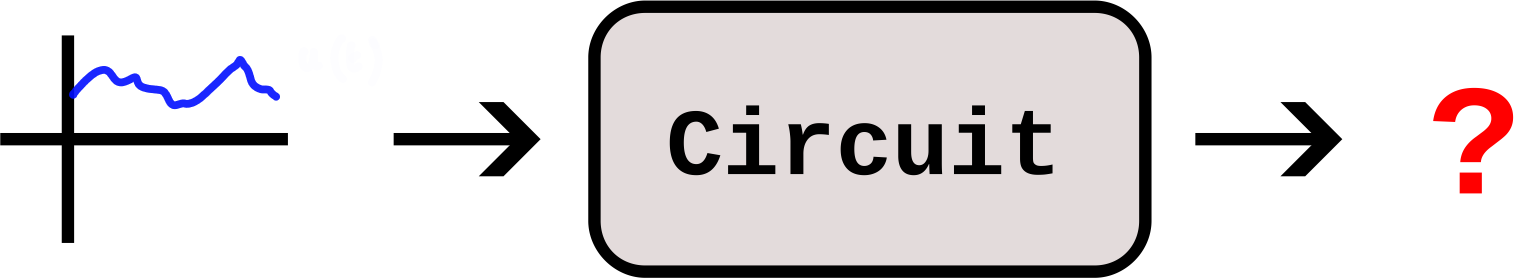
\includegraphics{part01/chap06/intro01.png}
\end{center}

C'est ici qu'intervient la transformée de Fourier. Au lieu de travailler directement sur le signal d'entrée, la transformée de Fourier nous dit que tout signal peut être décomposé comme une somme de signaux "élémentaires" sinusoïdaux. Notre approche peut donc être simplifiée : au lieu de calculer la réponse d'un circuit à un signal complexe, nous allons décomposer ce signal en une somme de sinusoïdes, puis étudier comment le filtre altère chacune d'entre elles. 

\begin{center}
\includesvg{part01/chap06/intro02}
\end{center}

Nous pourrons alors reconstruire la réponse en sommant les réponses élémentaires. 

\pagebreak
\section{Les séries de Fourier}

\subsection*{Définition}

Les séries de Fourier s'appliquent aux \textbf{\underline{fonctions périodiques}}. \\

Un signal périodique $s(t)$ de période $T$ peut, sous certaines conditions que nous supposerons toujours vérifiées en physique, se décomposer sous la forme suivante~:

\begin{equation}
	\bm{s(t) = a_0 + \sum_{n=1}^{\infty} \left(a_ncos\left( n\omega t\right) + b_nsin\left(n\omega t\right) \right)}
\end{equation}

Avec~: 

$$\omega=\dfrac{2\pi}{T}$$

et $a_0$, $a_n$, et $b_n$ des constantes~:

$$ a_0 = \dfrac{1}{T} \int_{0}^{T} s(t)dt $$

$$ a_n = \dfrac{2}{T} \int_{0}^{T} s(t)\,cos\left( n\omega t \right) dt \quad  \text{et} \quad b_n = \dfrac{2}{T} \int_{0}^{T} s(t)\,sin\left( n\omega t \right) dt $$  \\

\begin{itemize}
\item On peut remarquer que \textbf{le terme $a_0$ correspond à la valeur moyenne du signal}. \\

\item Les termes correspondant à $n=1$ sont appelés \textbf{le fondamental du signal}~:

$$ a_1\,cos\left( \omega t \right) + b_1\,sin\left( \omega t\right) $$  

\item Le terme général de rang $n$ est appelé \textbf{"harmonique de rang $n$"}~:

$$ a_n\,cos\left( n\omega t \right) + b_n\,sin\left( n\omega t\right) $$

\end{itemize}

\subsection*{Parité}

\begin{itemize}
\item Si la fonction s(t) est paire, tous les coefficients $b_n$ s'annulent :

$$ s(t) = \sum_{n=1}^{\infty} \left(a_ncos\left( n\omega t\right) \right) $$

\item Si la fonction s(t) est impaire, tous les coefficients $a_n$ s'annulent :

$$ s(t) = \sum_{n=1}^{\infty} \left(b_nsin\left(n \omega t\right) \right) $$

\end{itemize}

\subsection*{Forme phase-amplitude~:}

Le terme général $a_n cos( n \omega t ) + b_n sin( n \omega t )$ peut être réécrit sous la forme : 

$$ a_ncos(n\omega t)+b_nsin(n\omega t) = \sqrt{a_n^2+b_n^2}\left(\dfrac{a_n}{\sqrt{a_n^2+b_n^2}}\,cos(n\omega t) + \dfrac{b_n}{\sqrt{a_n^2+b_n^2}}\,sin(n\omega t)\right)$$

Si on pose~:

$$c_n = \sqrt{a_n^2+b_n^2} \quad\text{,}\quad tan(\phi_n) = \dfrac{b_n}{a_n} \quad\text{et}\quad cos(\phi_n)= \dfrac{a_n}{\sqrt{a_n^2+b_n^2}}$$

On obtient~:

$$ a_ncos(n\omega t)+b_nsin(n\omega t) = c_n cos( n \omega t - \phi_n ) $$ 

Et le signal s'écrit alors~:

\begin{equation}
\bm{s(t)= a_0 + \sum_{n=1}^{\infty} c_n cos( n \omega t - \phi_n )} 
\end{equation}

Cette écriture, par rapport à la précédente, présente l'intérêt de représenter notre signal comme une somme de termes de forme unique, en cosinus avec phase et amplitude, plutôt que comme une somme de termes de deux formes différentes. \\

\textbf{\underline{Note}}~: Le lecteur attentif aura remarqué une correspondance entre les coordonnées $(a_n,b_n)$, qui correspondent aux coodonnées cartésiennes d'un vecteur 2D, et les coordonnées $(c_n, \phi_n)$ qui correspondent aux coordonnées polaires de ce même vecteur. Nous allons continuer, dans les chapitres à venir, à exploiter cette correspondance entre signal sinusoïdal et vecteur (ou nombre complexe).

\subsection*{Forme exponentielle}

Une troisième forme existe pour les séries de Fourier. Il s'agit de la forme exponentielle qui s'écrit de la façon suivante~:

\begin{equation}
\bm{s(t) = \sum_{n=-\infty}^{\infty} d_n\,e^{jnwt} }
\end{equation}

Avec $j$ le nombre tel que $j^2=1$.

Dans cette forme, les coefficient $d_n$ sont des nombres complexes :

$$ d_n = \dfrac{1}{T} \int_{0}^{T} s(t)\,e^{ j\,n\,\omega\,t }\,dt \quad  \text{et donc} \quad d_n = 
\begin{cases} 
	\dfrac{a_n - j\,b_n}{2} & \text{si } n>0 \\
	\dfrac{a_n + j\,b_n}{2} & \text{si } n<0 \\
	a_0 & \text{si } n=0
\end{cases}
$$  

\subsection*{ Spectre en fréquence }

Le spectre en fréquence d'un signal $s(t)$ est obtenu en représentant les coefficients $a_n$, $b_n$ ou $c_n$ par rapport aux pulsations correspondantes~: \\

\begin{center}
\includesvg[scale=0.5]{part01/chap06/spectre_en_frequence}
\end{center}

Cette représentation graphique permet de représenter la décomposition d'un signal en ses harmoniques et d'en comprendre les composantes. \\

\textit{Exemple: Le signal carré}\\

On considère le signal carré de période $T$ et d'amplitude $E$ suivant~: 

\begin{center}
\includesvg{part01/chap06/signal_carre}
\end{center}

Le signal est symétrique et centré verticalement. On a donc~:

$$a_0 = 0$$

De plus, on remarque que le signal est impair. Les coefficient $a_n$ sont donc nuls. \\ Il reste donc uniquement les termes $b_n$ :

$$ b_n = \dfrac{2}{T} \int_{-T/2}^{T/2} u(t)\,sin(n\omega t)dt = \dfrac{2E}{n\pi} \left( 1 - cos(n\pi) \right) $$

La décomposition ne comprend donc que des harmoniques d'ordre impaire car le terme en cosinus s'annule pour n pair.\\

\begin{minipage}{0.4\textwidth}
\begin{center}
\includesvg{part01/chap06/spectre_carre}
\end{center}
\end{minipage}
\begin{minipage}{0.5\textwidth}
	$$ u(t) = \dfrac{4E}{\pi}\left[ sin(\omega t) + \dfrac{1}{3} sin ( 3\omega t ) + \dfrac{1}{5} sin( 5 \omega t ) \dots \right] $$
\end{minipage}\\

\bigskip

Le spectre du signal carré est caractérisé par une décroissance de l'amplitude des harmoniques en $1/n$, ce qui constitue une décroissante très lente. Cela est typique des fonctions présentant une ou plusieurs discontinuités. 

\begin{figure}[!h]
\centering
\begin{subfigure}{0.4\textwidth}
\begin{center}
\begin{gnuplot}[terminal=epslatex, terminaloptions={color dashed size 8cm,5cm}]
set sample 1000
set xzeroaxis linetype -1
set xtics border nomirror
set ytics border nomirror
set border 3
set xr [-0.09:1]
set yr [-1.5:1.50]
T = 1 
f = 1/T
pi = 3.14159
w = 2*pi*f 
E = 1
u(n,x) = 2*E/(n*pi)*( 1 - cos(n*pi) ) * sin( n*w*x)
f(k,x)= sum [n=1:k] u(n,x)
plot \
	f(3,x) w l lc 4 lw 6 t ''
\end{gnuplot}
\end{center}
\caption{$N=3$}
\end{subfigure}
\hfill
\begin{subfigure}{0.4\textwidth}
\begin{center}
\begin{gnuplot}[terminal=epslatex, terminaloptions={color dashed size 8cm,5cm}]
set sample 1000
set xzeroaxis linetype -1
set xtics border nomirror
set ytics border nomirror
set border 3
set xr [-0.09:1]
set yr [-1.5:1.50]
T = 1 
f = 1/T
pi = 3.14159
w = 2*pi*f 
E = 1
u(n,x) = 2*E/(n*pi)*( 1 - cos(n*pi) ) * sin( n*w*x)
f(k,x)= sum [n=1:k] u(n,x)
plot \
	f(10,x) w l lc 4 lw 6 t ''
\end{gnuplot}
\end{center}
\caption{$N=10$}
\end{subfigure}
\hfill
\begin{subfigure}{0.4\textwidth}
\begin{center}
\begin{gnuplot}[terminal=epslatex, terminaloptions={color dashed size 8cm,5cm}]
set sample 1000
set xzeroaxis linetype -1
set xtics border nomirror
set ytics border nomirror
set border 3
set xr [-0.09:1]
set yr [-1.5:1.50]
T = 1 
f = 1/T
pi = 3.14159
w = 2*pi*f 
E = 1
u(n,x) = 2*E/(n*pi)*( 1 - cos(n*pi) ) * sin( n*w*x)
f(k,x)= sum [n=1:k] u(n,x)
plot \
	f(50,x) w l lc 4 lw 6 t ''
\end{gnuplot}
\end{center}
	\caption{$N=50$}
\end{subfigure}
\hfill
\begin{subfigure}{0.4\textwidth}
\begin{center}
\begin{gnuplot}[terminal=epslatex, terminaloptions={color dashed size 8cm,5cm}]
set sample 1000
set xzeroaxis linetype -1
set xtics border nomirror
set ytics border nomirror
set border 3
set xr [-0.09:1]
set yr [-1.5:1.50]
T = 1 
f = 1/T
pi = 3.14159
w = 2*pi*f 
E = 1
u(n,x) = 2*E/(n*pi)*( 1 - cos(n*pi) ) * sin( n*w*x)
f(k,x)= sum [n=1:k] u(n,x)
plot \
	f(100,x) w l lc 4 lw 6 t ''
\end{gnuplot}
\end{center}
	\caption{$N=100$}
\end{subfigure}
\end{figure}

\subsection*{Phénomène de Gibbs}
\begin{minipage}{0.4\textwidth}
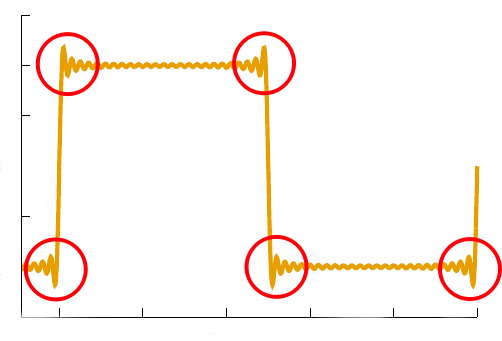
\includegraphics[width=\textwidth]{part01/chap06/gibbs.png}
\end{minipage}
\hfill
\begin{minipage}{0.5\textwidth}
\textbf{Le phénomène de Gibbs} est un effet de bord de la décomposition en séries de Fourier aux discontinuités. Ces "pics" oscillatoires (ringing) apparaissent en raison de l'approximation faite lorsque seules les N premières harmoniques du signal sont utilisées pour approximer un signal.\\

Lorsqu'un grand nombre d'harmoniques est pris en compte, cette erreur d'approximation converge vers une limite d'environ 9\% du changement de valeur.
\end{minipage}

\section{La transformée de Fourier}

La transformation de Fourier est une généralisation aux \textbf{\underline{fonctions non périodiques}} des séries de Fourier.

\subsection*{Définition}

La transformation de Fourier est une opération qui associe à chaque fonction intégrable sur ${\rm I\!R}$ une autre fonction décrivant le spectre fréquentiel de celle-ci. \\

Si elle existe, la transformée de Fourier de la fonction $f(t)$ s'écrit~:

\begin{equation}
	\begin{split}
		\mathcal{F}(f): \, & \mathbb{R} \rightarrow  \mathbb{C}  \\	
		& \xi \mapsto F(\xi)=\int_{-\infty}^{+\infty}f(t)\,e^{-j\,\xi\,t}\,dt \\
	\end{split}
\end{equation}

$F(\xi)$ indique la "quantité" de fréquence $\xi$ présente dans le signal $f(t)$ sur l'intervalle de temps $]-\infty;+\infty[$. \\

Il y a une équivalence entre donner $f(t)$ et donner $F(\xi)$ : ce sont deux descriptions équivalentes du même signal~:\\

\begin{itemize}

	\item L'une est \textbf{temporelle} \\

	\item L'autre est \textbf{fréquentielle} 

\end{itemize}

\subsection*{Transformée de Fourier inverse }

% FIXME

\subsection*{Spectre continu}

Le lecteur averti aura -je n'en doute pas- remarqué que la fonction $F(\xi)$ est à valeur complexe. Elle admet : \\

\begin{itemize}
	\item \textbf{un spectre d'amplitude}~:  

		$$A_\xi = \lvert F(\xi) \rvert $$ 

	\item \textbf{un spectre de phase}~: 

		$$\phi(\xi) = arg(\,F(\xi)\,)$$ \\

\end{itemize}

Ces spectres sont \underline{continus}, à la différence des spectres obtenus par les séries de Fourier qui étaient composés de raies calculées aux multiples de la fréquence fondamentale.


